\documentclass[a4paper, 11pt]{article}

% DEFINIËREN CODERING
\usepackage[utf8]{inputenc}

% DEFINIËREN BLAD
\usepackage[
top=20mm,
bottom=20mm,
left=20mm,
right=20mm,
heightrounded,
]{geometry}
\usepackage{lastpage}
\usepackage{fancyhdr}
%\pagestyle{fancy}
\fancyhead[L]{}
\fancyhead[C]{}
\fancyhead[R]{}
\fancyfoot[L]{}
\fancyfoot[C]{\thepage}
\fancyfoot[R]{}
\renewcommand{\headrulewidth}{0pt}
\renewcommand{\footrulewidth}{.4pt}
\setlength{\headheight}{13.6pt}
\setlength{\parindent}{1cm}

% MEDIA
% Tabellen
\usepackage{array}
\newcolumntype{L}[1]{>{\raggedright\let\newline\\\arraybackslash\hspace{0pt}}m{#1}}
\newcolumntype{C}[1]{>{\centering\let\newline\\\arraybackslash\hspace{0pt}}m{#1}}
\newcolumntype{R}[1]{<{\raggedleft\let\newline\\\arraybackslash\hspace{0pt}}m{#1}}
\usepackage{stackengine}
\newcommand\xrowht[2][0]{\addstackgap[.5\dimexpr#2\relax]{\vphantom{#1}}}
\usepackage{tabularx}
\usepackage{multirow}
\usepackage{hhline}
\usepackage{float}
% Afbeeldingen
\usepackage{graphicx}
% Figuren
\usepackage{tikz}

% WISKUNDE
% Basis
\usepackage{amsmath}
\usepackage{amssymb}
\usepackage{amsthm}
% Aanpassing
\usepackage{dsfont}   % Voor de natuurlijke, gehele, rationele, reële, complexe getallen => ``$\mathfb{}$''
\usepackage{mathdots} % Voor betere puntjes
\usepackage{esvect}   % Voor betere vectorpijltjes => ``$\vv{}$''
\usepackage{textcomp} % Nodig om gensymb correct te laten werken
\usepackage{gensymb}  % Invoegen van enkele symbolen => ``\degree ; \celcius ; \perthousand ; \ohm ; \micro''
\usepackage{cancel}   % Voor het beter doorstrepen van zaken => ``\cancel ; \bcancel ; \xcancel''
\usepackage{esint}    % Meervoudige kringintegralen

\newcommand{\naar}{\,$\rightarrow$\,}
\newcommand{\ppp}{\ldots}
\renewcommand{\empty}{$\varnothing$}
\newcommand{\of}{$\cup$}
\newcommand{\<}{\scriptsize\textless\normalsize}
\renewcommand{\>}{\scriptsize\textgreater\normalsize}

% Voorblad
\title{Programmeerproject 2:\\ Voorstudie Modeltrein Software Toepassing}
\date{Academiejaar 2024-2025}
\author{Jonas Br\"ull, 0587194\\ (Jonas.Simon.E.Brull@vub.be)\\\\ 2/3ba Computerwetenschappen}

% ==================================================================================================
\begin{document}

\pagenumbering{gobble}
\maketitle
\newpage

\pagenumbering{gobble}
\tableofcontents
\newpage

\pagestyle{fancy}
\setcounter{page}{1}
\pagenumbering{arabic}

% ==================================================================================================
\section{Introductie} % ============================================================================
Dit document beschrijft het ontwerp van de implementatie van een Modeltrein Software Toepassing in de programmeertaal Racket. Het is een deel van het opleidingsonderdeel ``Programmeerproject 2''.\\
\newline
Het onderwerp van het project is de ontwikkeling van een controlesysteem voor een modelspoor. De modeltreinen kunnen volledig digitaal aangestuurd worden door een extern programma aangestuurd met digitale commando’s. Digitale locomotieven gebruiken het elektrisch circuit op de sporen als een datacommunicatiebus. Niet alleen de snelheid van de locomotieven wordt op deze manier digitaal
geregeld, maar ook andere functionaliteiten zoals het veranderen van wissels\\
\newline
Tijdens deze opdracht wordt een controlesysteem ontwikkeld om modeltreinen aan te sturen. Het is de
bedoeling dat tegen het einde van het academiejaar een systeem ontwikkeld werd dat gebruikers
toelaat vanaf hun computer treinen over een modelspoor te laten rijden.\\
\newline
Het project bestaat uit drie grote componenten:
\begin{itemize}
	\item Een Command Station (Z21) dat de verschillende elementen van het modelspoor aanstuurt. Dit Command Station communiceert met de hardware via het Digital Command Control (DCC) protocol. De software hiervoor zit reeds ingebouwd in het Command Station. Het Command Station is aan te sturen door er via het netwerk commando’s naar te sturen door middel van de Z21-bibliotheek.
	\item Infrabel is de component die instaat voor de communicatie tussen de software en de
	modelbouwhardware (detectie van treinen en aansturing van treinen en wissels) en het
	doorlopend beheer van de infrastructuur (bv. automatisch remsysteem). Dit is deel van de infrastructuur en moet permanent draaien. Infrabel kan draaien op een computer of op een Raspberry Pi (een kleine gelimiteerde computer).
	\item NMBS en de grafische interface (GUI). NMBS staat in voor de functionaliteit die geen
	logisch onderdeel is van de infrastructuur maar er bovenop bouwt, zoals een grafische
	interface, het uitstippelen van trajecten of het opstellen van tijdstabellen. NMBS draait
	op je eigen computer en communiceert met Infrabel. Naar het einde van het project toe
	zal die communicatie via een netwerkverbinding (TCP) dienen te gebeuren.
\end{itemize}
Zowel de Infrabel module, als de Provider module zullen steunen op een railway module, deze de fysieke spoorwegopstelling (of diens simulator) modeleert en deze steeds dezelfde staat zal hebben.
\newpage

% ==================================================================================================
\section{Railway} % ================================================================================
De railway-module houdt ten allen tijden de staat van de fysieke modelspoorweg bij. Deze module bestaat uit verschillende atomaire abstracties van de verschillende hardware-componenten, die de modelspoorweg bezit, deze allemaal aangestuurd worden vanuit de main-klasse.

\subsection{Main} % ++++++++++++++++++++++++++++++++++++++++++++++++++++++++++++++++++++++++++++++++
De \texttt{Main} klasse is het startpunt van railway-module van de software en functioneert tevens ook als een interface. Om een digitaal equivalent van de staat van de modelspoorweg bij te houden, bezit deze klasse hiervoor ook de nodige getters en setters. Deze klasse berekent zelf welke spoorwegsegmenten bezet zijn en welke vrij, aan de hand van de locatie van de treinen. Hierdoor is het niet mogelijk om de status van spoorwegsegmenten, detectieblokken en wissels aan te passen. Om botsingen te voorkomen, is het well mogelijk deze te reserveren.
\begin{table}[H]
	\begin{center}
		\begin{tabular}{|l l l|}
			\hline
			\textbf{Naam} & \textbf{Signatuur} & \textbf{Uitleg}\\
			\hline
			\texttt{make-object} & (\textit{pair} \naar \textit{Main}) & Constructor\\
			\hline
			\texttt{get-ajacent} & (\textit{symbol} \naar \textit{pair}) & Geeft lijst van alle \lq buren' van een segment\\
			\texttt{get-crossing-ids} & (\empty \naar \textit{pair}) & Geeft lijst van overwegen\\
			\texttt{get-crossing-state} & (\textit{symbol} \naar \textit{symbol}) & Geeft status weer van gegeven overweg\\
			\texttt{set-crossing-state!} & (\textit{symbol} \textit{symbol} \naar \empty) & Update gegeven overweg naar gegeven status\\
			\texttt{get-detection-block-ids} & (\empty \naar \textit{pair}) & Geeft lijst van detectie blokken\\
			\texttt{get-detection-block-state} & (\textit{symbol} \naar \textit{symbol}) & Geeft status weer van gegeven detectieblok\\
			\texttt{reserve-detection-block!} & (\textit{symbol} \naar \empty) & Reserveert gegeven detectieblok\\
			\texttt{get-light-ids} & (\empty \naar \textit{pair}) & Geeft lijst van lichten\\
			\texttt{get-light-signal} & (\textit{symbol} \naar \textit{symbol}) & Geeft signaal weer van gegeven licht\\
			\texttt{set-light-signal!} & (\textit{symbol} \textit{symbol} \naar \empty) & Update gegeven licht met gegeven signaal\\
			\texttt{get-segment-ids} & (\empty \naar \textit{pair}) & Geeft lijst van segmenten\\
			\texttt{get-segment-state} & (\textit{symbol} \naar \textit{symbol}) & Geeft status weer van gegeven segment\\
			\texttt{reserve-segment!} & (\textit{symbol} \naar \empty) & Reserveert gegeven spoorwegsegment\\
			\texttt{get-switch-ids} & (\empty \naar \textit{pair}) & Geeft lijst van wissels\\
			\texttt{get-switch-position} & (\textit{symbol} \naar \textit{symbol}) & Geeft postitie weer van gegeven wissel\\
			\texttt{set-switch-position!} & (\textit{symbol} \textit{symbol} \naar \empty) & Update gegeven wissel met gegeven positie\\
			\texttt{reserve-switch!} & (\textit{symbol} \naar \empty) & Reserveert gegeven wissel\\
			\texttt{get-train-ids} & (\empty \naar \textit{pair}) & Geeft lijst van treinen\\
			\texttt{get-train-speed} & (\textit{symbol} \naar \textit{symbol}) & Geeft snelheid weer van gegeven trein\\
			\texttt{set-train-speed!} & (\textit{symbol} \textit{symbol} \naar \empty) & Update gegeven trein met gegeven snelheid\\
			\hline
		\end{tabular}
		\caption{Operaties van de Railway/Main klasse}
	\end{center}
\end{table}

\subsection{Crossing} % ++++++++++++++++++++++++++++++++++++++++++++++++++++++++++++++++++++++++++++
De \texttt{Crossing} klasse is de atomaire abstractie van een spoorwegoverweg.
\begin{table}[H]
	\begin{center}
		\begin{tabular}{|l l l|}
			\hline
			\textbf{Naam} & \textbf{Signatuur} & \textbf{Uitleg}\\
			\hline
			\texttt{make-object} & (\textit{symbol} \naar \textit{Crossing}) & Constructor\\
			\hline
			\texttt{get-state} & (\empty \naar \textit{symbol}) & Geeft de status van de overweg\\
			\texttt{set-state!} & (\textit{symbol} \naar \empty) & Verandert de status van de overweg, waardoor deze opent/sluit\\
			\hline
		\end{tabular}
		\caption{Operaties van de Railway/Crossing klasse}
	\end{center}
\end{table}

\newpage

\subsection{Detection-block} % +++++++++++++++++++++++++++++++++++++++++++++++++++++++++++++++++++++
De \texttt{Detection-block} klasse is de atomaire abstractie van een detectieblok. Deze is een uitbreiding van de \texttt{Segment} klasse.
\begin{table}[H]
	\begin{center}
		\begin{tabular}{|l l l|}
			\hline
			\textbf{Naam} & \textbf{Signatuur} & \textbf{Uitleg}\\
			\hline
			\texttt{make-object} & (\textit{symbol} \naar \textit{Detection-block}) & Constructor\\
			\hline
			\texttt{get-state} & (\empty \naar \textit{symbol}) & Geeft de status van het detection block\\
			\texttt{set-state!} & (\textit{symbol} \naar \empty)& Update de status van het detection block\\
			\hline
		\end{tabular}
		\caption{Operaties van de Railway/Detection-block klasse}
	\end{center}
\end{table}

\subsection{Light} % +++++++++++++++++++++++++++++++++++++++++++++++++++++++++++++++++++++++++++++++
De \texttt{Light} klasse is de atomaire abstractie van een licht.
\begin{table}[H]
	\begin{center}
		\begin{tabular}{|l l l|}
			\hline
			\textbf{Naam} & \textbf{Signatuur} & \textbf{Uitleg}\\
			\hline
			\texttt{make-object} & (\textit{symbol} \naar \textit{Light}) & Constructor\\
			\hline
			\texttt{get-signal} & (\empty \naar \textit{symbol}) & Geeft het signaal van het Light\\
			\texttt{set-signal!} & (\textit{symbol} \naar \empty) & Update het signaal van het Light\\
			\hline
		\end{tabular}
		\caption{Operaties van de Railway/Light klasse}
	\end{center}
\end{table}

\subsection{Segment} % +++++++++++++++++++++++++++++++++++++++++++++++++++++++++++++++++++++++++++++
De \texttt{Segment} klasse is de atomaire abstractie van een spoorwegsegment.
\begin{table}[H]
	\begin{center}
		\begin{tabular}{|l l l|}
			\hline
			\textbf{Naam} & \textbf{Signatuur} & \textbf{Uitleg}\\
			\hline
			\texttt{make-object} & (\textit{symbol} \naar \textit{Segment}) & Constructor\\
			\hline
			\texttt{get-state} & (\empty \naar \textit{symbol}) & Geeft de status van het segment\\
			\texttt{set-state!} & (\textit{symbol} \naar \empty) & Update de status van het segment\\
			\hline
		\end{tabular}
		\caption{Operaties van de Railway/Segment klasse}
	\end{center}
\end{table}

\subsection{Switch} % ++++++++++++++++++++++++++++++++++++++++++++++++++++++++++++++++++++++++++++++
De \texttt{Switch} klasse is de atomaire abstractie van een spoorwegwissel.
\begin{table}[H]
	\begin{center}
		\begin{tabular}{|l l l|}
			\hline
			\textbf{Naam} & \textbf{Signatuur} & \textbf{Uitleg}\\
			\hline
			\texttt{make-object} & (\textit{symbol} \naar \textit{Switch}) & Constructor\\
			\hline
			\texttt{get-position} & (\empty \naar \textit{symbol}) & Geeft de status van de wissel\\
			\texttt{set-position!} & (\textit{symbol} \naar \empty) & Update de status van de wissel\\
			\hline
		\end{tabular}
		\caption{Operaties van de Railway/Switch klasse}
	\end{center}
\end{table}

\newpage

\subsection{Switch-3way} % +++++++++++++++++++++++++++++++++++++++++++++++++++++++++++++++++++++++++
De \texttt{Switch-3way} klasse is de atomaire abstractie van een spoorwegwissel deze van 3 sporen laat samenkomen tot 1 spoor. Deze klasse is een uitbreiding is van de \texttt{Switch} klasse.
\begin{table}[H]
	\begin{center}
		\begin{tabular}{|l l l|}
			\hline
			\textbf{Naam} & \textbf{Signatuur} & \textbf{Uitleg}\\
			\hline
			\texttt{make-object} & (\textit{symbol} \naar \textit{Switch-3way}) & Constructor\\
			\hline
			\texttt{get-position} & (\empty \naar \textit{symbol}) & Geeft de status van de wissel\\
			\texttt{set-position!} & (\textit{symbol} \naar \empty) & Update de status van de wissel\\
			\hline
		\end{tabular}
		\caption{Operaties van de Railway/Switch klasse}
	\end{center}
\end{table}

\subsection{Switch-cross} % ++++++++++++++++++++++++++++++++++++++++++++++++++++++++++++++++++++++++
De \texttt{Switch-cross} klasse is de atomaire abstractie van een spoorwegwissel deze de kruising maakt tussen 2 keer 2 sporen. Deze klasse is een uitbreiding van de \texttt{Switch} klasse.
\begin{table}[H]
	\begin{center}
		\begin{tabular}{|l l l|}
			\hline
			\textbf{Naam} & \textbf{Signatuur} & \textbf{Uitleg}\\
			\hline
			\texttt{make-object} & (\textit{symbol} \naar \textit{Switch-cross}) & Constructor\\
			\hline
			\texttt{get-position} & (\empty \naar \textit{symbol}) & Geeft de status van de wissel\\
			\texttt{set-position-1!} & (\textit{symbol} \naar \empty) & Update de status van het eerste paar in de wissel\\
			\texttt{set-position-2!} & (\textit{symbol} \naar \empty) & Update de status van het tweede paar in de wissel\\
			\hline
		\end{tabular}
		\caption{Operaties van de Railway/Switch klasse}
	\end{center}
\end{table}

\subsection{Train} % +++++++++++++++++++++++++++++++++++++++++++++++++++++++++++++++++++++++++++++++
De \texttt{Train} klasse is de atomaire abstractie van een trein.
\begin{table}[H]
	\begin{center}
		\begin{tabular}{|l l l|}
			\hline
			\textbf{Naam} & \textbf{Signatuur} & \textbf{Uitleg}\\
			\hline
			\texttt{make-object} & (\empty \naar \textit{Train}) & Constructor\\
			\hline
			\texttt{get-location} & (\empty \naar \textit{symbol}) & Geeft terug op welk segment/detectie-blok/wissel de trein is\\
			\texttt{get-next-location} & (\empty \naar \textit{symbol}) & Geeft volgende segment/detectie-blok/wissel van de trein\\
			\texttt{get-train-speed} & (\empty \naar \textit{symbol}) & Geeft de snelheid van de trein\\
			\texttt{set-train-speed!} & (\textit{symbol} \naar \empty) & Update de snelheid van de trein\\
			\hline
		\end{tabular}
		\caption{Operaties van de Railway/Train klasse}
	\end{center}
\end{table}

\newpage

% ==================================================================================================
\section{Provider} % ===============================================================================
De Provider-module is een abstractie van de software die gebruikt kan worden door clienten (bijvoorbeeld NMBS). Deze module is verantwoordelijk voor het beheren van routes op het treinnetwerk, moet ervoor zorgen dat klanten correcte timetables hebben en het moet mogelijk zijn om na een crash de huidige staat van de fysieke spoorweg terug te krijgen.

\subsection{Main} % ++++++++++++++++++++++++++++++++++++++++++++++++++++++++++++++++++++++++++++++++
De \texttt{Main} klasse is het startpunt van de module en tevens ook de interface naar andere modules toe. De module bestaat uit twee onafhankelijke delen, een Grafische User Interface (GUI) en de interne logica (Logic), waar de main-klasse de interface speelt tussen de twee.
\begin{table}[H]
	\begin{center}
		\begin{tabular}{|l l l|}
			\hline
			\textbf{Naam} & \textbf{Signatuur} & \textbf{Uitleg}\\
			\hline
			\texttt{make-object} & (\empty \naar \textit{Provider}) & Constructor\\
			\hline
			\texttt{get-x} & (\textit{symbol} \naar \empty) & Placeholder voor getters voor uitwisseling van informatie\\
			\texttt{set-x!} & (\empty \naar \textit{symbol}) & Placeholder voor setters voor updaten van informatie\\
			\hline
		\end{tabular}
		\caption{Operaties van de Provider/Main klasse}
	\end{center}
\end{table}

\subsection{GUI} % +++++++++++++++++++++++++++++++++++++++++++++++++++++++++++++++++++++++++++++++++

\subsubsection{Startup} % --------------------------------------------------------------------------
De \texttt{Startup} klasse is de grafische representatie van het opstart menu, waar onder andere de configuratie voor de TCP verbinding zal kunnen gebeuren.
\begin{table}[H]
	\begin{center}
		\begin{tabular}{|l l l|}
			\hline
			\textbf{Naam} & \textbf{Signatuur} & \textbf{Uitleg}\\
			\hline
			\texttt{make-object} & (\empty \naar \textit{Startup}) & Constructor\\
			\hline
		\end{tabular}
		\caption{Operaties van de Provider/GUI/Startup klasse}
	\end{center}
\end{table}

\subsubsection{Command\&Control} % -----------------------------------------------------------------
De \texttt{Command\&Control} klasse is de grafische user interface deze module, de gebruikers van de Provider zullen hier de volledige applicatie meer kunnen besturen.
\begin{table}[H]
	\begin{center}
		\begin{tabular}{|l l l|}
			\hline
			\textbf{Naam} & \textbf{Signatuur} & \textbf{Uitleg}\\
			\hline
			\texttt{make-object} & (\empty \naar \textit{C\&C}) & Constructor\\\hline
			\texttt{update!} & (\empty \naar \empty) & Update de GUI naar de nieuwe staat van het systeem\\
			\hline
		\end{tabular}
		\caption{Operaties van de Provider/GUI/Command\&Control klasse}
	\end{center}
\end{table}

\newpage

\subsection{Logic} % +++++++++++++++++++++++++++++++++++++++++++++++++++++++++++++++++++++++++++++++

\subsubsection{App} % ------------------------------------------------------------------------------
De \texttt{App} klasse staat in voor de interne logica van het provider-systeem. Verschillende functies worden gedelegeerd naar de verschillende klasses waar deze op steunt.
\begin{table}[H]
	\begin{center}
		\begin{tabular}{|l l l|}
			\hline
			\textbf{Naam} & \textbf{Signatuur} & \textbf{Uitleg}\\
			\hline
			\texttt{make-object} & (\empty \naar \textit{App}) & Constructor\\
			\hline
			\texttt{get-x} & (\textit{symbol} \naar \empty) & Placeholder voor getters voor uitwisseling van informatie\\
			\texttt{set-x!} & (\empty \naar \textit{symbol}) & Placeholder voor setters voor updaten van informatie\\
			\hline
		\end{tabular}
		\caption{Operaties van de Provider/Logic/App klasse}
	\end{center}
\end{table}

\subsubsection{Startup} % --------------------------------------------------------------------------
De \texttt{Startup} klasse is verantwoordelijk voor alle logica die gepaart gaat met het opstarten van de applicatie
\begin{table}[H]
	\begin{center}
		\begin{tabular}{|l l l|}
			\hline
			\textbf{Naam} & \textbf{Signatuur} & \textbf{Uitleg}\\
			\hline
			\texttt{make-object} & (\empty \naar \textit{Startup}) & Constructor\\
			\hline
			\texttt{get-x} & (\textit{symbol} \naar \empty) & Placeholder voor getters voor uitwisseling van informatie\\
			\texttt{set-x!} & (\empty \naar \textit{symbol}) & Placeholder voor setters voor updaten van informatie\\
			\hline
		\end{tabular}
		\caption{Operaties van de Provider/Logic/Startup klasse}
	\end{center}
\end{table}

\subsubsection{TCP} % ------------------------------------------------------------------------------
De \texttt{TCP} klasse is verantwoordelijk voor de communicatie met de Infrabel module.
\begin{table}[H]
	\begin{center}
		\begin{tabular}{|l l l|}
			\hline
			\textbf{Naam} & \textbf{Signatuur} & \textbf{Uitleg}\\
			\hline
			\texttt{make-object} & (\empty \naar \textit{TCP}) & Constructor\\
			\hline
			\texttt{send-message} & (\textit{string} \naar \empty) & Verstuur een bericht naar de Infrabel module\\
			\hline
		\end{tabular}
		\caption{Operaties van de Provider/Logic/TCP klasse}
	\end{center}
\end{table}

\subsubsection{Route-calculator} % -----------------------------------------------------------------
De \texttt{Route-calculator} klasse is verantwoordelijk voor het berekenen van de korste route tussen twee segmenten.
\begin{table}[H]
	\begin{center}
		\begin{tabular}{|l l l|}
			\hline
			\textbf{Naam} & \textbf{Signatuur} & \textbf{Uitleg}\\
			\hline
			\texttt{make-object} & (\empty \naar \textit{Route-calculator}) & Constructor\\
			\hline
			\texttt{calculate-shortest-between} & (\textit{symbol} \textit{symbol} \naar \textit{pair}) & Berekent kortste route\\
			\hline
		\end{tabular}
		\caption{Operaties van de Provider/Logic/Route-calculator klasse}
	\end{center}
\end{table}

\newpage

\subsubsection{Concurrency} % ----------------------------------------------------------------------
De \texttt{Concurrency} klasse is verantwoordelijk voor het opstaan en inladen van de software.
\begin{table}[H]
	\begin{center}
		\begin{tabular}{|l l l|}
			\hline
			\textbf{Naam} & \textbf{Signatuur} & \textbf{Uitleg}\\
			\hline
			\texttt{make-object} & (\empty \naar \textit{Concurrency}) & Constructor\\
			\hline
			\texttt{save} & (\textit{string} \naar \empty) & Slaat huidige staat van de software op.\\
			\texttt{load!} & (\textit{string} \naar \empty) & Laadt de staat van de software in van een bestand.\\
			\hline
		\end{tabular}
		\caption{Operaties van de Provider/Logic/Concurrency klasse}
	\end{center}
\end{table}

\subsubsection{Timetables} % -----------------------------------------------------------------------
De \texttt{Timetables} klasse is verantwoordelijk voor het genereren van tijdstabellen.
\begin{table}[H]
	\begin{center}
		\begin{tabular}{|l l l|}
			\hline
			\textbf{Naam} & \textbf{Signatuur} & \textbf{Uitleg}\\
			\hline
			\texttt{make-object} & (\empty \naar \textit{Timetables}) & Constructor\\
			\hline
			\texttt{generate-timetable} & (\textit{symbol} \naar \textit{pair}) & Genereert timetables voor trein\\
			\hline
		\end{tabular}
		\caption{Operaties van de Provider/Logic/Timetables klasse}
	\end{center}
\end{table}

% ==================================================================================================
\section{Infrabel} % ===============================================================================
De Infrabel-module is verantwoordelijk voor het beheren van het treinnetwerk, moet ervoor zorgen dat het volledige netwerk aangestuurt kan worden en dat dit veilig gebeurt.

\subsection{Main} % ++++++++++++++++++++++++++++++++++++++++++++++++++++++++++++++++++++++++++++++++
De \texttt{Main} klasse is het startpunt van de module en tevens ook de interface naar andere modules toe. De module bestaat uit twee onafhankelijke delen, een Grafische User Interface (GUI) en de interne logica (Logic), waar de main-klasse de interface speelt tussen de twee.
\begin{table}[H]
	\begin{center}
		\begin{tabular}{|l l l|}
			\hline
			\textbf{Naam} & \textbf{Signatuur} & \textbf{Uitleg}\\
			\hline
			\texttt{make-object} & (\empty \naar \textit{Main}) & Constructor\\
			\hline
			\texttt{get-x} & (\textit{symbol} \naar \empty) & Placeholder voor getters voor uitwisseling van informatie\\
			\texttt{set-x!} & (\empty \naar \textit{symbol}) & Placeholder voor setters voor updaten van informatie\\
			\hline
		\end{tabular}
		\caption{Operaties van de Infrabel/Main klasse}
	\end{center}
\end{table}

\subsection{GUI} % +++++++++++++++++++++++++++++++++++++++++++++++++++++++++++++++++++++++++++++++++

\subsubsection{Startup} % --------------------------------------------------------------------------
De \texttt{Startup} klasse is de grafische representatie van het opstart menu, waar onder andere de configuratie voor de TCP verbinding zal kunnen gebeuren.
\begin{table}[H]
	\begin{center}
		\begin{tabular}{|l l l|}
			\hline
			\textbf{Naam} & \textbf{Signatuur} & \textbf{Uitleg}\\
			\hline
			\texttt{make-object} & (\empty \naar \textit{Startup}) & Constructor\\
			\hline
		\end{tabular}
		\caption{Operaties van de Infrabel/GUI/Startup klasse}
	\end{center}
\end{table}

\newpage

\subsubsection{Admin-debug} % ----------------------------------------------------------------------
De \texttt{Admin-debug} klasse is de grafische user interface deze module, de programmeurs van Infrabel zullen hier de volledige applicatie meer kunnen besturen.
\begin{table}[H]
	\begin{center}
		\begin{tabular}{|l l l|}
			\hline
			\textbf{Naam} & \textbf{Signatuur} & \textbf{Uitleg}\\
			\hline
			\texttt{make-object} & (\empty \naar \textit{Admin-debug}) & Constructor\\
			\hline
			\texttt{update!} & (\empty \naar \empty) & Update de GUI naar de nieuwe staat van het systeem\\
			\hline
		\end{tabular}
		\caption{Operaties van de Provider/GUI/Admin-debug klasse}
	\end{center}
\end{table}

\subsection{Logic} % +++++++++++++++++++++++++++++++++++++++++++++++++++++++++++++++++++++++++++++++

\subsubsection{App} % ------------------------------------------------------------------------------
De \texttt{App} klasse is verantwoordelijk voor de interne logica van de Infrabel module. Het besteet verschillende taken uit aan de klasses waarop deze steunt.
\begin{table}[H]
	\begin{center}
		\begin{tabular}{|l l l|}
			\hline
			\textbf{Naam} & \textbf{Signatuur} & \textbf{Uitleg}\\
			\hline
			\texttt{make-object} & (\empty \naar \textit{App}) & Constructor\\
			\hline
			\texttt{get-x} & (\textit{symbol} \naar \empty) & Placeholder voor getters voor uitwisseling van informatie\\
			\texttt{set-x!} & (\empty \naar \textit{symbol}) & Placeholder voor setters voor updaten van informatie\\
			\hline
		\end{tabular}
		\caption{Operaties van de Provider/Logic/App klasse}
	\end{center}
\end{table}

\subsubsection{Startup} % --------------------------------------------------------------------------
De \texttt{Startup} klasse is verantwoordelijk voor alle logica die gepaart gaat met het opstarten van de applicatie
\begin{table}[H]
	\begin{center}
		\begin{tabular}{|l l l|}
			\hline
			\textbf{Naam} & \textbf{Signatuur} & \textbf{Uitleg}\\
			\hline
			\texttt{make-object} & (\empty \naar \textit{Startup}) & Constructor\\
			\hline
			\texttt{get-x} & (\textit{symbol} \naar \empty) & Placeholder voor getters voor uitwisseling van informatie\\
			\texttt{set-x!} & (\empty \naar \textit{symbol}) & Placeholder voor setters voor updaten van informatie\\
			\hline
		\end{tabular}
		\caption{Operaties van de Provider/Logic/App klasse}
	\end{center}
\end{table}

\subsubsection{TCP} % ------------------------------------------------------------------------------
De \texttt{TCP} klasse is verantwoordelijk voor de communicatie met de Provider module.
\begin{table}[H]
	\begin{center}
		\begin{tabular}{|l l l|}
			\hline
			\textbf{Naam} & \textbf{Signatuur} & \textbf{Uitleg}\\
			\hline
			\texttt{make-object} & (\empty \naar \textit{TCP}) & Constructor\\
			\hline
			\texttt{send-message} & (\textit{string} \naar \empty) & Verstuur een bericht naar de Provider module\\
			\hline
		\end{tabular}
		\caption{Operaties van de Provider/Logic/TCP klasse}
	\end{center}
\end{table}

\newpage

\subsubsection{UDP} % ------------------------------------------------------------------------------
De \texttt{UDP} klasse is een abstractie bovenop ofwel de Z21, ofwel de simulator. Aangezien het mogelijk moet blijven om op beiden te steunen, wordt de abstractie gemaakt.
\begin{table}[H]
	\begin{center}
		\begin{tabular}{|l l l|}
			\hline
			\textbf{Naam} & \textbf{Signatuur} & \textbf{Uitleg}\\
			\hline
			\texttt{make-object} & (\empty \naar \textit{UDP}) & Constructor\\
			\hline
			\texttt{start} & (\empty \naar \empty) & Start simulator / hardware.\\
			\texttt{stop} & (\empty \naar \empty) & Stopt simulatie / hardware.\\
			\texttt{add-loco} & (\textit{symbol} \textit{symbol} \textit{symbol} \naar \empty) & Voegt locomotief toe.\\
			\texttt{get-loco-speed} & (\textit{symbol} \naar \textit{number}) & Geeft snelheid locomotief.\\
			\texttt{set-loco-speed!} & (\textit{symbol} \textit{number} \naar \empty) & Update snelheid locomotief.\\
			\texttt{get-detection-block-ids} & (\empty \naar \textit{pair}) & Geeft lijst van detectieblokken.\\
			\texttt{get-occupied-detection-blocks} & (\empty \naar \textit{pair}) & Geeft lijst bezette detectieblokken.\\
			\texttt{get-switch-ids} & (\empty \naar \textit{pair}) & Geeft lijst van wissels.\\
			\texttt{get-switch-position} & (\textit{symbol} \naar \textit{number}) & Geeft positie van opgegeven wissel.\\
			\texttt{set-switch-position!} & (\textit{symbol} \textit{number} \naar \empty) & Update positie van opgegeven wissel.\\
			\texttt{open-crossing!} & (\textit{symbol} \naar \empty) & Opent opgegeven overweg.\\
			\texttt{close-crossing!} & (\textit{symbol} \naar \empty) & Sluit opgegeven overweg.\\
			\texttt{set-sign-code!} & (\textit{symbol} \textit{symbol} \naar \empty) & Updatet opgegeven licht.\\
			\hline
		\end{tabular}
		\caption{Operaties van de Provider/Logic/UDP klasse}
	\end{center}
\end{table}

\subsubsection{Collision-detector} % ---------------------------------------------------------------
De \texttt{Collision-detector} klasse is verantwoordelijk voor het voorkomen van botsingen.
\begin{table}[H]
	\begin{center}
		\begin{tabular}{|l l l|}
			\hline
			\textbf{Naam} & \textbf{Signatuur} & \textbf{Uitleg}\\
			\hline
			\texttt{make-object} & (\empty \naar \textit{Collision-detector}) & Constructor\\
			\hline
			\texttt{calculate-collision?} & (\textit{symbol} \textit{symbol} \naar \textit{boolen}) & Returnt mogelijke botsingen\\
			\hline
		\end{tabular}
		\caption{Operaties van de Provider/Logic/Collision-detector klasse}
	\end{center}
\end{table}

\subsubsection{Signalisator} % ---------------------------------------------------------------------
De \texttt{Signalisator} klasse is verantwoordelijk dat alle signalisatie rondom de spoorweg correct is.
\begin{table}[H]
	\begin{center}
		\begin{tabular}{|l l l|}
			\hline
			\textbf{Naam} & \textbf{Signatuur} & \textbf{Uitleg}\\
			\hline
			\texttt{make-object} & (\empty \naar \textit{Signalisator}) & Constructor\\
			\hline
			\texttt{update!} & (\textit{string} \naar \empty) & Update klasse met huidige staat spoorweg\\
			\hline
		\end{tabular}
		\caption{Operaties van de Provider/Logic/Signalisator klasse}
	\end{center}
\end{table}

\subsubsection{Concurrency} % ----------------------------------------------------------------------
De \texttt{Concurrency} klasse is verantwoordelijk voor het opstaan en inladen van de software.
\begin{table}[H]
	\begin{center}
		\begin{tabular}{|l l l|}
			\hline
			\textbf{Naam} & \textbf{Signatuur} & \textbf{Uitleg}\\
			\hline
			\texttt{make-object} & (\empty \naar \textit{Concurrency}) & Constructor\\
			\hline
			\texttt{save} & (\textit{string} \naar \empty) & Slaat huidige staat van de software op.\\
			\texttt{load!} & (\textit{string} \naar \empty) & Laadt de staat van de software in van een bestand.\\
			\hline
		\end{tabular}
		\caption{Operaties van de Provider/Logic/Concurrency klasse}
	\end{center}
\end{table}

\newpage

% ==================================================================================================
\section{Afhankelijkheidsdiagram} % ================================================================
\begin{center}
	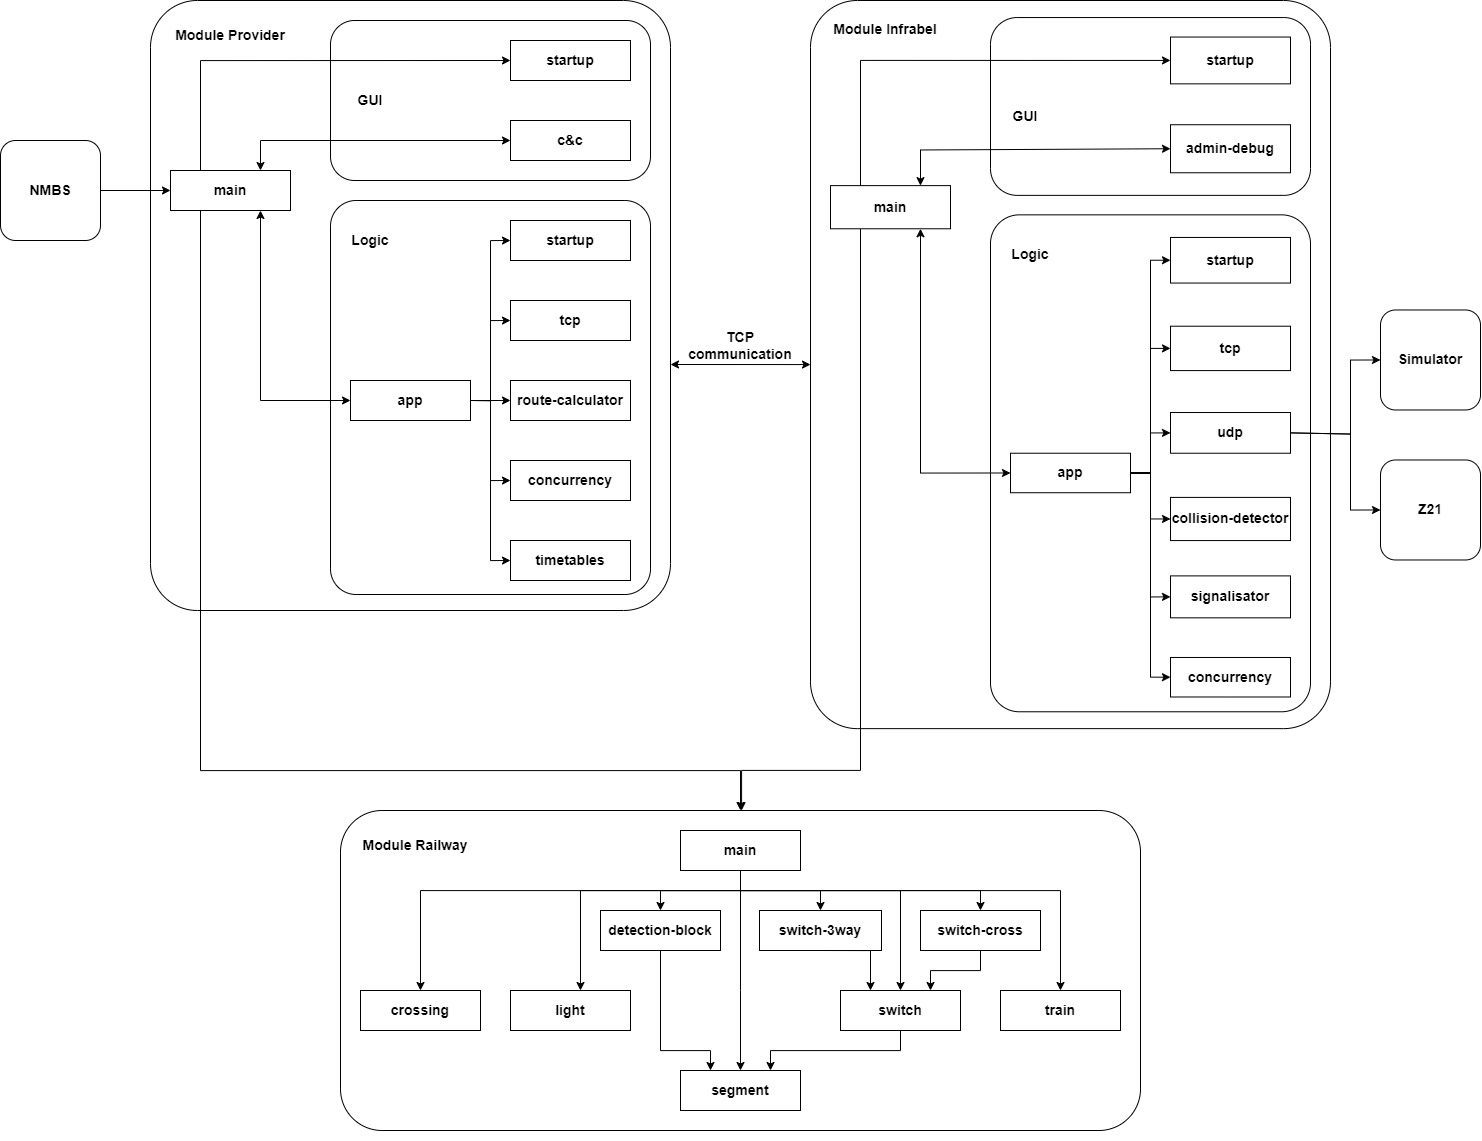
\includegraphics[scale=.33]{Afhankelijkheidsdiagrammen/2024-2025.jpg}
\end{center}

\newpage

% ==================================================================================================
\section{Planning} % ===============================================================================
Volgens het Agile-Scrum model, gezien zoals in Software Engineering uit de derde bachelor, ga ik het bouwen van het software systeem opsplitsen in een opeenvolging van 1 week durende sprints.
\begin{table}[H]
	\begin{center}
		\begin{tabular}{|l l|}
			\hline
			\textbf{Week} & \textbf{Actie} \\
			\hline
			week 5: 20/10 & \textbf{Indienen voorstudie}\\
			week 6 & Sprint 1: Railway module bouwen + testen + documentatie\\
			week 6: 25/10& \emph{WPO: feedback voorstudie en voorbereiding fase 1}\\
			week 7 & Sprint 2: Infrabel logica bouwen + testen + documentatie\\
			week 8 & Sprint 3: Provider logica bouwen + testen + documentatie\\
			week 9 & Sprint 4: GUI provider bouwen + testen + documentatie\\
			week 9: 12/11 & \emph{WPO: massaprogrammeren fase 1}\\
			\hline
			week 9: 17/11 & EIGEN DEADLINE FASE 1\\
			week 10 & (week van Saint-V, voorbereidingen evenement)\\
			week 11: & Troubleshooting + testing + documentatie\\
			week 11: 01/12 & \textbf{Deadline fase 1}\\
			\hline
			week 12 & (week van Vrijzinnig Zangfeest, voorbereidingen evenement)\\
			week 13: & Voorbereiding fase 2, inhalen eventuele tekorten\\
			week 13: 13/12 & \emph{WPO: feedback fase 1 en voorbereiding fase 2}\\
			week 14: & Voorbereiding examens\\
			\hline
			\hline
			week 15-16 & (Blok: wintervakantie)\\
			week 17-20 & \emph{Examenperiode}\\
			week 21 & (lesvrije week)\\
			\hline
			\hline
			week 22 & Sprint 5: TCP splitsing Provider Infrabel+ testen + documentatie\\
			week 23 & Sprint 6: Implementatie botspreventie + testen + documentatie\\
			week 23-24 & \emph{WPO: massaprogrammeren fase 2}\\
			week 24 & Sprint 7: Implementatie hardware + testen + documentatie\\
			week 25 & Sprint 8: Implementatie hardware + testen + documentatie\\
			\hline
			week 25: 09/03 & EIGEN DEADLINE FASE 2\\
			week 26  & Troubleshooting + testing + documentatie\\
			week 26: 16/03 & \textbf{Deadline fase 2}\\
			week 27-28 & Voorbereiding fase 3, inhalen eventuele tekorten\\
			week 28: & \textbf{Mondelinge verdediging fase 2}\\
			\hline
			week 29 & Sprint 9: Automatische trajectberekening + testen + documentatie\\
			week 30-31 & (Blok: lentevakantie)\\
			week 32 & Sprint 10: \\
			week 32-33: & \emph{WPO: massaprogrammeren fase 3}\\
			week 33 & Sprint 11: Automatische trajectberekening + testen + documentatie\\
			week 34 & Sprint 12: Extra vereisten + testen + documentatie\\
			week 35 & Sprint 13: Extra vereisten + testen + documentatie\\
			\hline
			week 35: 18/05 & EIGEN DEADLINE FASE 3\\
			week 36 & Troubleshooting + testing + documentatie\\
			week 36: 25/05 & \textbf{Deadline fase 3}\\
			examenperiode & \textbf{Mondelinge verdediging fase 3}\\
			\hline
		\end{tabular}
		\caption{Planning Modeltrein Software Toepassing}
	\end{center}
\end{table}

% ==================================================================================================
\label{lastpage}
\end{document}

%
% OPMERKINGEN OP VOORSTUDIE
%
% Algemeen:
% - Denk al eens na over de uitgebreide vereiste.
% 
% ADT’s:
% - Het graphics ADT beschrijft niet goed wat het verschil is met het GUI ADT.
% - Het wpo over tcp zal pas in de derde fase georganiseerd worden.
%
% Indien je toch al meer te weten wilt komen over de tcp verbinding kun je altijd de racket documentatie lezen (https://docs.racket-lang.org/reference/tcp.html).
% - Switch ADT: In jouw switch ADT zijn er 2 posities mogelijk. Hoe zal
% dit ADT omgaan met S-2-3 die 3 posities heeft?
% - Waarom slaat het train ADT niet de richting en snelheid van de trein op?
% - Voor automatische traject berekening is het de bedoeling dat een traject wordt berekend. Het is dus niet de bedoeling om een overzicht van alle korste routes bij te houden.
% - Waarom gebruik je stations als stopplaatsen en niet de detectieblokken als stopplaatsen?
% 
% Afhankelijkheidsdiagram en software-architectuur:
% OK - De GUI mag niet afhankelijk zijn van NMBS.
% OK - ADT-stop mag niet afhankelijk zijn van het ADT-positie aangezien dit ADT zich in infrabel bevindt.
% OK - Heel veel van jouw ADTs zijn wederzijds afhankelijk. Dit zal ervoor zorgen dat het minder makkelijk is om code later aan te passen. Probeer dus meer in lagen te werken waarbij een laag afhankelijk is van de laag eronder.
% 
% OK Planning:
% OK - Vergeet geen testen te schrijven.
%
